
\documentclass[11pt]{amsart}
\usepackage{geometry}                % See geometry.pdf to learn the layout options. There are lots.
\geometry{letterpaper}                   % ... or a4paper or a5paper or ... 
%\geometry{landscape}                % Activate for for rotated page geometry
%\usepackage[parfill]{parskip}    % Activate to begin paragraphs with an empty line rather than an indent
\usepackage{graphicx}
\usepackage{amssymb}
\usepackage{epstopdf}
\usepackage{listings}
\usepackage{latexsym}
\usepackage{algorithmic}
\usepackage{algorithm}
\usepackage{times}
\usepackage{mdwlist}
\usepackage{fancybox}
\usepackage{shadow}
\usepackage{rotating}
\usepackage{subfigure}
\usepackage{epsfig}
\usepackage{url}
\usepackage{color}
\usepackage{setspace}

\DeclareGraphicsRule{.tif}{png}{.png}{`convert #1 `dirname #1`/`basename #1 .tif`.png}

\title{Course Project}
\author{Mostafa Abdulla Uddin\\
UID: 00899812}
%\date{}                                           % Activate to display a given date or no date

\begin{document}
\begin{titlepage}

\begin{center}
\vspace*{2in}
\textsc{\LARGE EnergySniffer:  Using Audio and Magnetic sensor}\\[1.5cm]
\textsc{\Large Course Project}\\[0.5cm]

\vspace*{2in}
\begin{minipage}{0.4\textwidth}
\begin{flushleft} \large
\emph{Student:}\\
Mostafa Abdulla \textsc{Uddin}\\
UID: 00899812\\
\end{flushleft}
\end{minipage}
\begin{minipage}{0.4\textwidth}
\begin{flushright} \large
\emph{Instructor:} \\
Dr. Tamer \textsc{Nadeem}
\end{flushright}
\end{minipage}


\vfill

{\large \today}
\end{center}

\end{titlepage}


\section{Usage/Targeted Audience}

EnergySniffer is an home energy usage monitoring application based on smartphone sensors reading. The main objective of this project is to exploit the sensors in smartphones to detect usage of home appliances. From that usage and the detection of machine can help us to measure energy usage by that machine. However, as a part of this project, we have only exploited the Audio and Magnetic sensor for this project. As these sensors in smartphones are not powerful enough to monitor the usage of machine, so we conduct some research to identify the challenges of using the sensors in smartphone for detecting energy usage. 

EnergySniffer project was intially targeted to the Customers. However, later we make this project much more research oriented. So the outcomes of this project is some research analysis and challenges to implement EnergySniffer project. During this project we have hacked the Android phone to understand the operation of both Audio and Magnetic sensor. Also the audio processing and machine learning algorithm was implemented in native code C/C++ at Kernel level for better performance. Providing this source code as an efficient API for the future developer and researcher.

\section{ Motivation}
\begin{itemize*}
\item Home Energy Monitoring: About 21\% of US energy is consumed by house. Energy Usage at House has an increasing trend. So monitoring the energy usage at house creates awareness among people to consume less energy and have more control over energy usage.
\item Sensors in SmartPhone: Now a days smartphones come with lots of sensors. Utilizing these sensors in innovative way is an interesting area of research. Using these sensors for monitoring energy usage at house is an ambitious thinking. But this ambitious idea creates something interesting research findings.
\item Flexible and Cheap: Utilizing the sensors of smartphone for energy monitoring could provide a chip and flexible solution to current complex solution of energy monitoring.

\end{itemize*}

\section{Component/Modules/Use cases/}

Following is the flow chart diagram of the main component of the EnergySniffer System. It has mainly two components i) Offline Learning and ii) Online detecting. In offline learning it collects the sensor data to build models and in online detecting it detects the model based on capturing real sensor data [Figure \ref{fig:flowchart} ].

  
\begin{figure}[htb]
\begin{center}
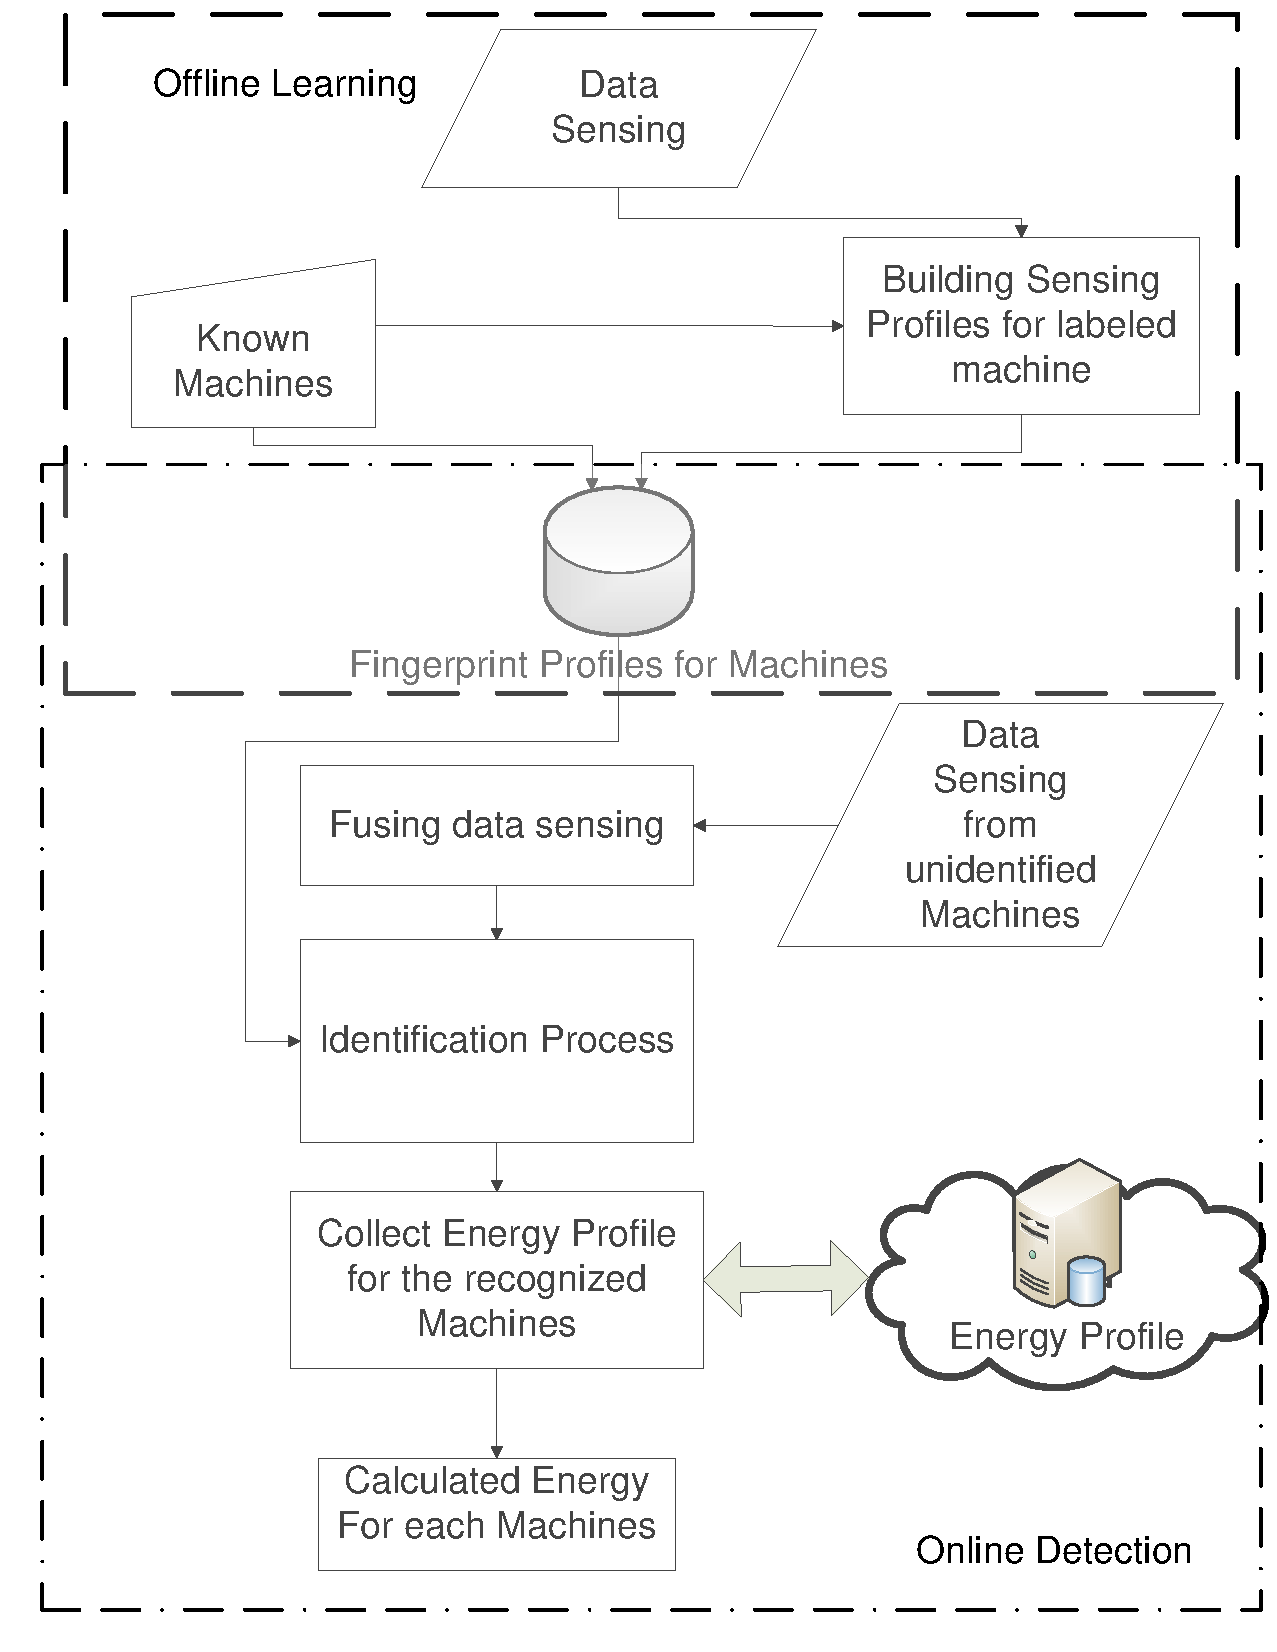
\includegraphics[width=1.0\linewidth, angle = 0]{Flowchart.pdf}
\caption{Complete Flow chart of EnergySniffer System} \label{fig:flowchart}
\end{center}
\end{figure}

In this project we fully implemented the Audio sensor data to collect the acoustic sensor data to build probabilistic generative models for different machine and then we use those model to detect running machines 




The Screen shot of the testing application is in figure \ref{fig:screenshot}

\begin{figure}[htb]
\begin{center}
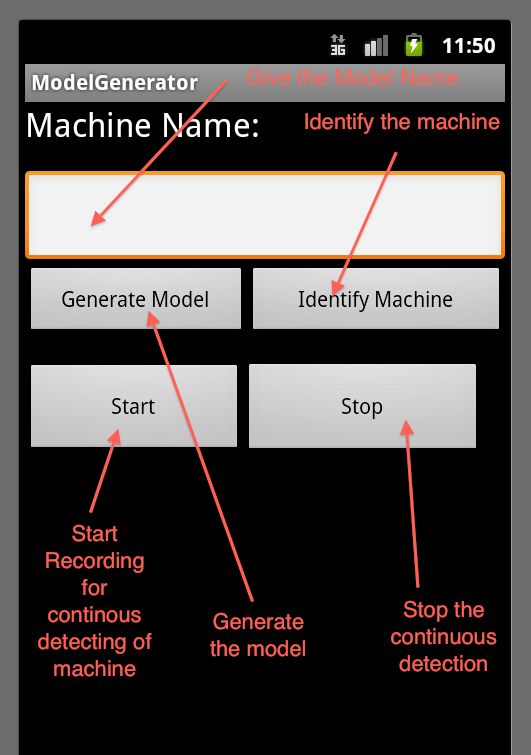
\includegraphics[width=1.0\linewidth, angle = 0]{screenshot.png}
 \label{fig:screenshot}
\end{center}
\end{figure}

\section{Team role Assignment}
Team Task assignment is shown in table \ref{tab:assign}.

\begin{table}[htb]
\centering
\scalebox{1.0}{
\begin{tabular}{|l|c|}
\hline
Task & Assigned To\\
\hline
FFT/Signal Processing/MFCC feature Implementation & Mostafa\\
Machine learning/ Model Implementation & Mostafa\\
Machine detection implementation & Mostafa\\
\hline
Magnetic Sesnsor Research & Mostafa\\
Collecting Magnetic Sensor Data at driver level & Mostafa\\
\hline
\end{tabular}
}
\caption{Task Assignment.}
\label{tab:assign}
\end{table}

\section{Lessor Learned or Observation}

\subsection{Audio Sensor}

We implemented our prototype system and tested in our lab office[ figure \ref{fig:lablayout}].


\begin{figure}[htb]
\begin{center}
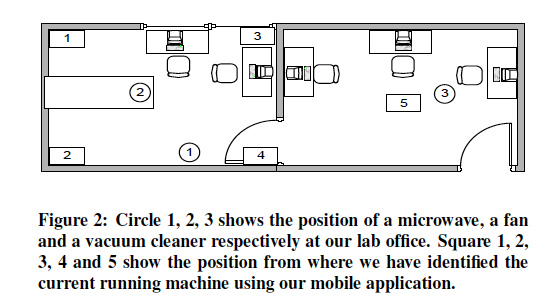
\includegraphics[width=1.0\linewidth, angle = 0]{lablayout.png}
\label{fig:lablayout}
\end{center}
\end{figure}

Following are some result of using Audio sensor data to detect machines [Figure \ref{fig:result1}, \ref{fig:result2}, \ref{fig:result3} ]
\begin{figure}[htb]
\begin{center}
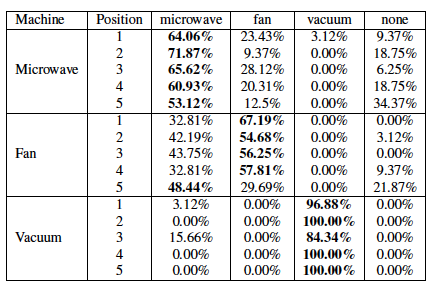
\includegraphics[width=1.0\linewidth, angle = 0]{result1.png}
\label{fig:result1}
\end{center}
\end{figure}

\begin{figure}[htb]
\begin{center}
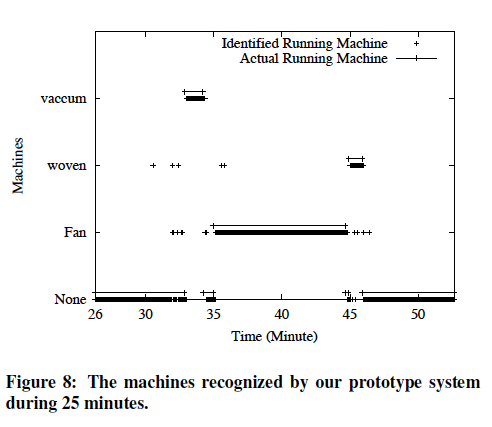
\includegraphics[width=1.0\linewidth, angle = 0]{result2.png}
\label{fig:result2}
\end{center}
\end{figure}


\begin{figure}[htb]
\begin{center}
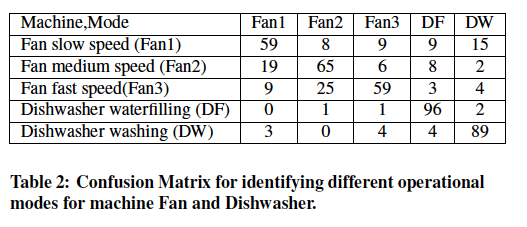
\includegraphics[width=1.0\linewidth, angle = 0]{result3.png}
\label{fig:result3}
\end{center}
\end{figure}

In Audio Sensor experiment we were not able to detect multiple machine at a time. Also We found that signal processing taken a huge amount of processing time, which make the detection technique difficult. So We are now implementing the FFT/Signal processing and machine learning algorithm in Android OS.

\subsection{Magnetic Sensor}

When we take the magnetic sensor of the smartphone close to some running machine we saw following behavior. When the machine is turned on magnetic sensor reading shows rapid variation in data. Magnetic sensor of the smartphone measure the strength of earth magnetic field in three axis. However due to other magnetic device or electromagnetic activities the magnetic sensor reading shows some fluctuation or interference [figure \ref{fig:magnetic1}, \ref{fig:magnetic1}].

\begin{figure}[htb]
\begin{center}
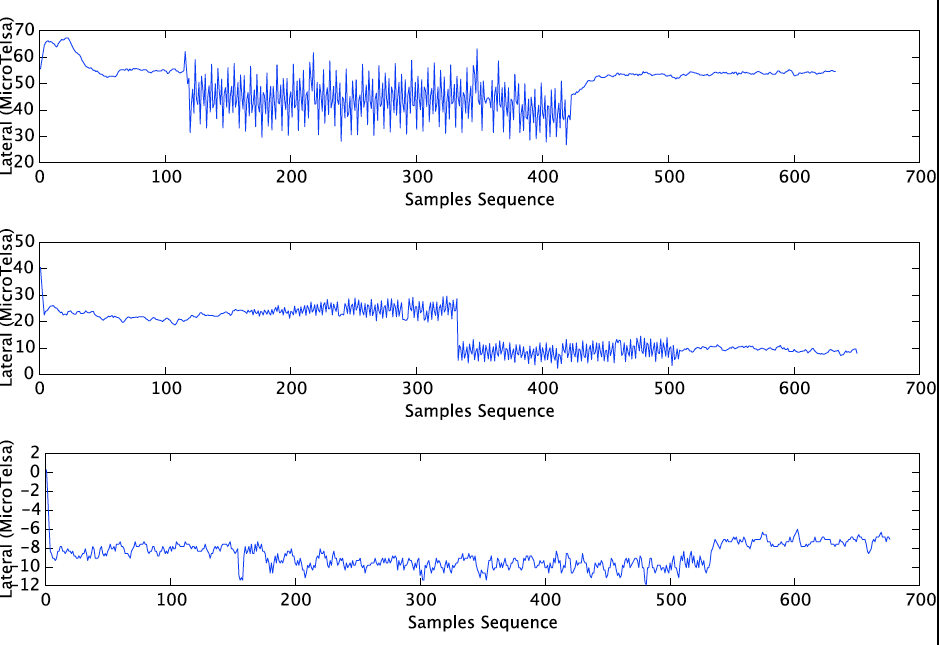
\includegraphics[width=1.0\linewidth, angle = 0]{magnetic1.png}
\caption{Magnetic Sensor data Reading for Three Machine} \label{fig:magnetic1}
\end{center}
\end{figure}


\begin{figure}[htb]
\begin{center}
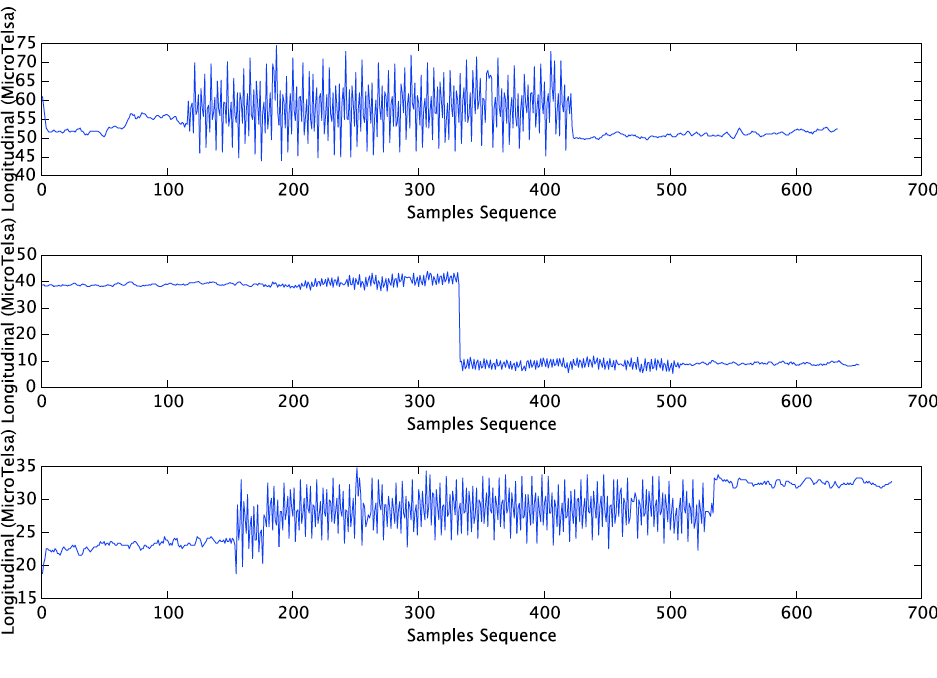
\includegraphics[width=1.0\linewidth, angle = 0]{magnetic2.png}
\caption{Magnetic Sensor data Reading for Three Machine} \label{fig:magnetic2}
\end{center}
\end{figure}

The magnetic sensor itself runs a very low bandwidth low pass filtering over the collected data. Magnetic sensor is embedded with the smartphone to detect the orientation of the smartphone screen and for calculating electronic compass. For both this purpose the magnetic field of the earth needs to be determined accurately and should be resistive to background interference noise. Thats why this sensor in smartphone use a very low bandwidth low pass filtering to make the data DC and to remove all high frequency interference. Which make it worse for developing our application on measuring electric power consume by a running machine [Figure \ref{fig:magnetic3}].


\begin{figure}[htb]
\begin{center}
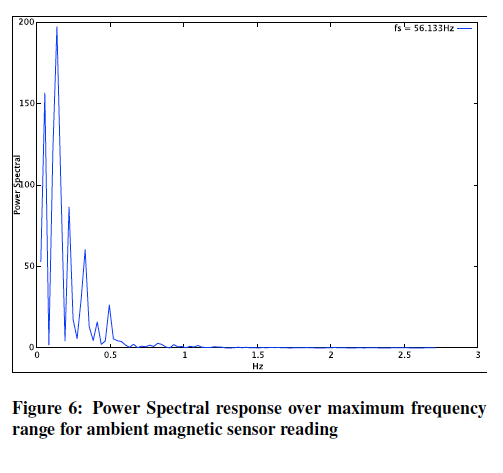
\includegraphics[width=1.0\linewidth, angle = 0]{magnetic3.png}
\label{fig:magnetic3}
\end{center}
\end{figure}

\section{Future Work}

Following are points that we want to keep in mind to implement it in future.
\begin{itemize*}
\item We want to build complete Signal processing and important machine learning technique as  a libraries for Android OS. For future Researcher.
\item To do some research about how this large number of sensor data should be collected and processed
\item Research on android phone audio driver libraries.
\item Research on magnetic sensor libraries. To add an additional magnetic sensor with the Android phone for measuring the current or energy in power line.
\end{itemize*}

\end{document}  